\chapter{Mixture regression surrogate}

\section{Gaussian mixture regression}
Taking a convex combination of a set of multivariate Gaussian distributions is a Gaussian mixture model
$$p(z) = \sum_{k=1}^K \pi_k \mathcal{N}(z|\mu_k, \Sigma_k)$$  
Defining $z := (x,y)$ we can model our data, as a generative model $p(x,y)$, now, since the conditonal 
of a Gaussain mixture again is Gaussain mixture - i.e. closed form expression, we can exactly calculate
$p(y|x) = GMM_{y|x}$

Assuming iid data the likelihood is given as 
$$p(\mathcal{D}|\mu_1, \dots, \mu_K, \Sigma_1, \dots, \Sigma_K, \pi_1, \dots, \pi_K) = \prod_{i=1}^n \sum_{k=1}^K \pi_k \mathcal{N}(z_i|\mu_k, \Sigma_k)$$
And the log likelihood, 
$$\log p(\mathcal{D}| ..) = \sum_{i=1}^n \log \sum_{k=1}^K \pi_k \mathcal{N}(z_i|\mu_k, \Sigma_k)$$


\subsection*{Dealing with wrong variance}
\begin{figure}[H]%
    \centering
    {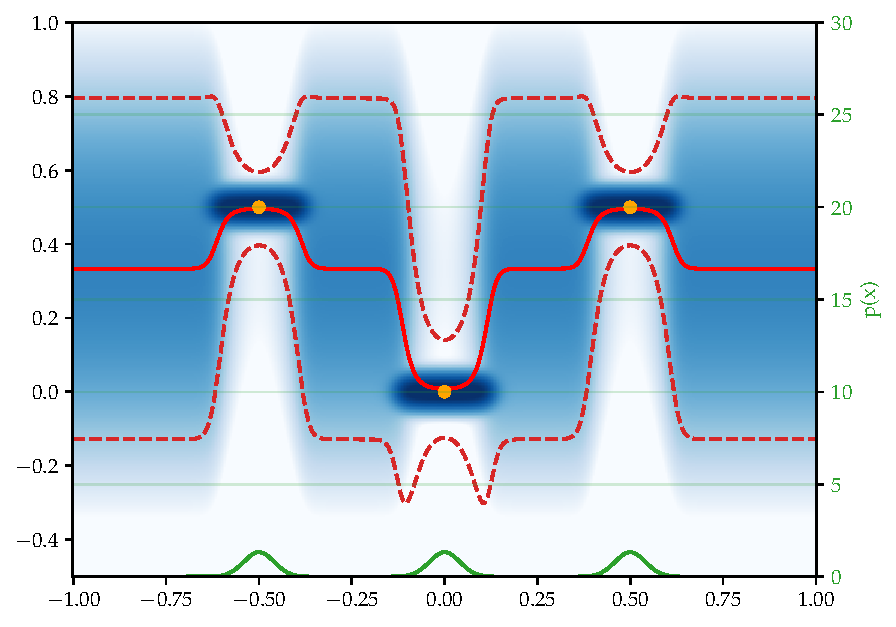
\includegraphics[width=0.46\textwidth]{Pictures/mixture_regression_variance_problem1.pdf} }%
    \qquad
   {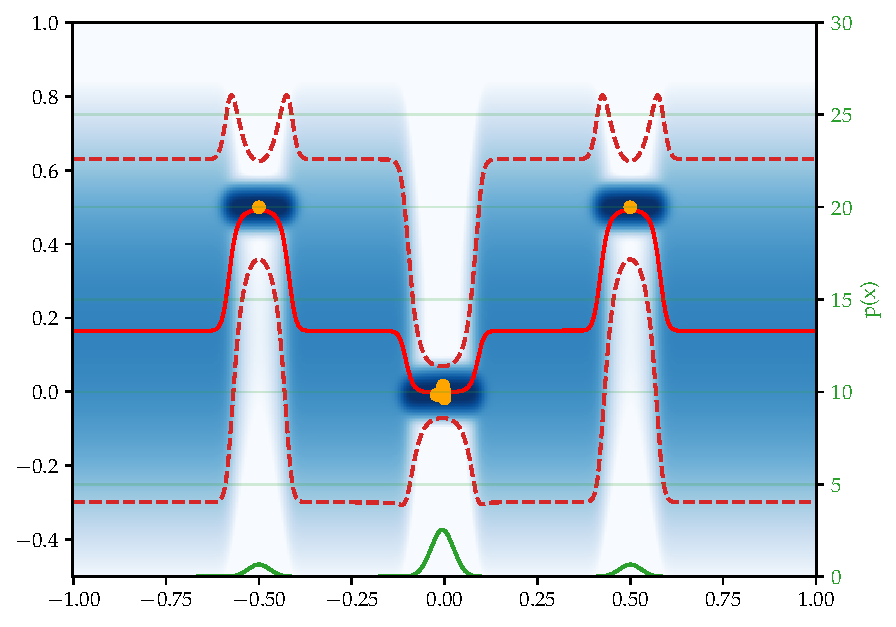
\includegraphics[width=0.46\textwidth]{Pictures/mixture_regression_variance_problem2.pdf} }%
   \qquad
   {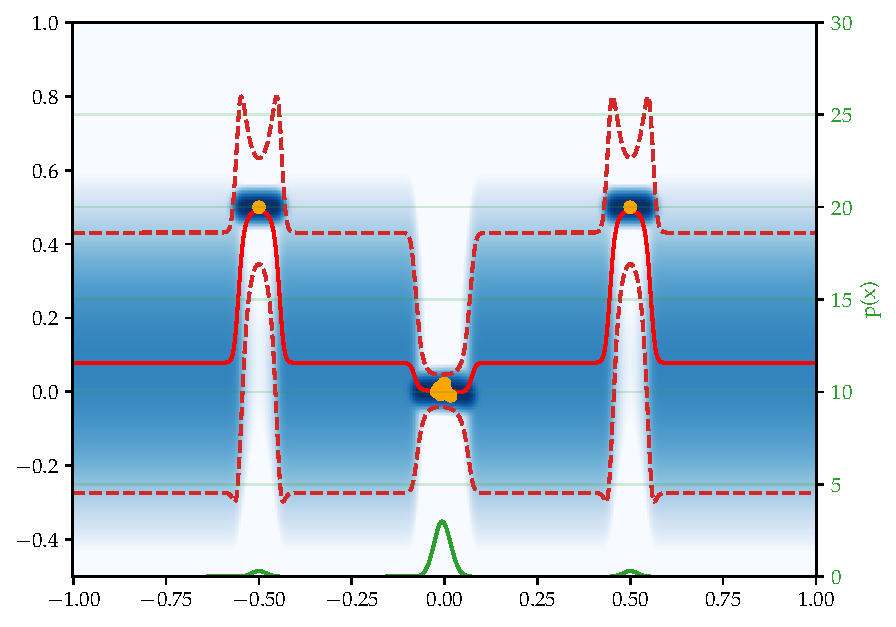
\includegraphics[width=0.46\textwidth]{Pictures/mixture_regression_variance_problem3.pdf} }%
   \caption{EI improvement might in this case be stucked at the point 0,
    since the conditional distribution is normalized by $p(x)$ and therefore not
    influenced by the amount of data}%
    \label{MixtureReg_challenge}%
\end{figure}


<variance manipulation>
<Expected improvement manipulation>


\section{Mixture regression in a Bayesian setting}
As seen in examples. The uncertainty of conditional distribution is way too certain
in areas with no data points, therefore we need to enhance the model with some bayesian 
flavour. 

$$p(y|x,\mathcal{D}) = p(y|x,Z)p(Z|x)$$



\subsection*{Expetation-maximization algorithm}
A way to find local maxima in the likehood function is using the EM algorithm. 

If we define a latent/hiddem random variabel $Z_i \in \{1,\dots, K\}$ for each data point, then 
the likelihood function becomes, 
$$L(\theta|\mathcal{D}, Z) = \prod_{i=1}^n \sum_{k=1}^K 1(Z_i = k) \pi_k \mathcal{N}(z_i|\mu_k, \Sigma_k)$$

Now the expectation wrt. the current value $p(Z|\mathcal{D}, \theta^k)$ is given as 
$$Q(\theta|\theta^k) = \mathcal{E}_{p(Z|\mathcal{D}, \theta^k)}=L(\theta|\mathcal{D}, Z) $$

And then update the next parameter estimate with
$$\theta^{k+1} = \arg \max_{\theta} Q(\theta|\theta^k)$$

This is repeated untill convergence. 


\section{Sum product networks}
We will for a large extend just see SPN as a large mixture model. This is a totally valid observation. 

\subsection*{Mixture model}
%from [@desana]:
\begin{definition} 
    A sub-network $\bar S_z$ of $S$ is an SPN, which includes the root $S$ and then includes nodes
    according to the following recursive scheme: 
\end{definition}
\begin{algorithm}[H]
    \caption*{Collection of sub-network $S_z$ of $S$}\label{SPN4}
    \begin{algorithmic}
    %\State \textbf{Global:}  $S_z$ 
    \Function{Process}{node i, $S_z$}
    \If{$i \in \mathcal{L}eaf(S)$}
        \State  $\textbf{return: }$ 
    \EndIf
    %\For{$i \in I_{o}$}
    \If{$i\in \mathcal{S}um(S)$}
       %\State $S_z =S_z \cup \{j \in ch(i)\}$ \Comment{include one child of node $i$}
        \State $S_z =S_z.add(j \in ch(i))$ \Comment{include one child of node $i$}
        \State $\textbf{return: } \text{Process}(j, S_z)$
    \EndIf
    \If{$i\in \mathcal{P}rod(S)$}
        \State $S_z =S_z \cup \{j | j \in ch(i)\}$ \Comment{include all childen of node $i$}
        \For{$j \in ch(i)$}
            \State $\textbf{return: } \text{Process}(j,S_z)$
        \EndFor
    \EndIf
    \State $\textbf{return: } S_z$
    \EndFunction
    \State $S_z =  \text{Process(root,Ø)}$
    \end{algorithmic}
\end{algorithm}
So we see that at each sum node the number of different sub-networks multiplies with the number of children for that
sum node. And thereby, the total number of sub-networks is
 $$Z = \prod_{i\in \mathcal{S}um(S)}|ch(i)|$$ 
 i.e. an exponential large amount of sub-networks. This is the amount of
 mixture components implicitly defined in an SPN. 
 Denote the set of edges in the sub-network $\mathcal{E}(S_z)$.
Now the we define a mixture coeficient, $\lambda_z$ and component for each $S_z$ as 
$$\lambda_z := \prod_{(i,j)\in \mathcal{E}(S_z)} w_{i,j}, \hspace{1cm}
p_z(x,y|\theta) := \prod_{i \in \mathcal{L}(S_z)} p_i(x,y)$$
where $p_i(x,y)$ is the leaf distribution at leaf node $i$ paramitised with $\theta$. 
It can now be proven that the SPN can be interpreted as the following mixture model, 
$$p(x,y|w,\theta) = \sum_{z=1}^Z \lambda_z(w)p_z(x,y|\theta)$$
i.e. by the weighted sum of all $Z$ sub-networks. For convinience
we define each sum component as $p(z,x,y|w,\theta) := \lambda_z(w)p_z(x,y|\theta)$.
Evaluation of $p(x,y|w,\theta)$ will never be done as the sum over $Z$ components, 
instead there is a proposition. 

\begin{proposition}
    Consider a SPN, S, a sum node $q \in \mathcal{S}um(S)$ and a child $i \in ch(q)$,
    then the following relation holds, 
    $$\sum_{z:(q,i)\in \mathcal{E}(S_z)} \lambda_z(w) p_z(x,y|\theta) = w_{i,q}
    \frac{\partial S}{\partial v(q)} v(i)$$
\end{proposition}



\subsection*{Conditional of SPN}

We will soon see how it is possible to write the conditional distribution as the mixture, 
$$p(y|x) = \sum_{z \in \Sigma(S)} \gamma(x) p_{z_y}(y)$$
where $ \Sigma(S)$ is the set of all sub-networks in the SPN, $S$ - \todo{IT IS EXPONENTIALLY LARGE}.  
And where $p_{z_y}(y)$ is defined through $p_z(x,y)$, 
\begin{align*}
    p_z(x,y) &= \prod_{l \in \mathcal{L}eaf(z_x)} \phi_l(x)\prod_{l \in \mathcal{L}eaf(z_y)} \phi_l(y)\\
            &=: p_{z_x}(x) p_{z_y}(y) 
\end{align*}
where $\phi_l$ is the density of the $l$'th leafs tractable distribution. Recall that we can interpret an SPN
as the mixture model, 
$$p(x,y) = \sum_{z \in \Sigma(S)} \lambda_z p_z(x,y)$$
where $\lambda_z = \prod_{(q,j) \in \mathcal{E}(z)} w_{q,j}$. First we calculate the marginal density,
$p(x)$, 
\begin{align*}
    p(x) &= \int p(x,y)dy\\
    &= \int \sum_{z \in \Sigma(S)} \lambda_z p_z(x,y)dy\\
    %&= \sum_{z \in \Sigma(S)} \lambda_z  \int p_z(x,y)dy\\
    &= \sum_{z \in \Sigma(S)} \lambda_z p_{z_x}(x)\int p_{z_y}(y)dy \\
    &= \sum_{z \in \Sigma(S)} \lambda_z p_{z_x}(x)
\end{align*}
Now we are ready to calculate the conditional density, 
\begin{align*}
    p(y|x) &=  \frac{p(x,y)}{p(x)}\\
            &= \frac{\sum_{z \in \Sigma(S)} \lambda_z p_z(x,y)}{p(x)}\\
            &=\sum_{z \in \Sigma(S)}\frac{ \lambda_z p_{z_x}(x)}{p(x)} p_{z_y}(y)\\
            &=\sum_{z \in \Sigma(S)}\frac{ \lambda_z p_{z_x}(x)}{\sum_{z \in \Sigma(S)} \lambda_z p_{z_x}(x)} p_{z_y}(y)\\
            &=\sum_{z \in \Sigma(S)} \gamma(x) p_{z_y}(y)
\end{align*}
So we defined $\gamma(x) = \frac{ \lambda_z p_{z_x}(x)}{\sum_{z \in \Sigma(S)} \lambda_z p_{z_x}(x)}$ 
and this is very convinient, as we will see soon is 
equavalent to the derivative of the log-likehood
of the SPN, which is easily obtained by automatic differentiation. 

\subsection*{calculation of $\gamma(x)$}
expectation maximization of a mixture model, is given by Bishop..
the responsibility of a datapoint to belong to one mixture component, is given by
$$\gamma(z_{nk}) = \frac{w_k p_j(x_n)}{\sum_i w_i p_i(x_n)}$$
We can prove that the responsibility is equal to the gradient of the log likehood, 
$$L:= \sum_n \log \sum_j w_j \exp \psi_j(x_n)$$
where we define $\psi_j(x_n) = \log p_j(x_n)$. Take the gradient 
$$\frac{\partial L}{\partial \psi_{j}(x_{n})} = \frac{w_k p_j(x_n)}{\sum_i w_i p_i(x_n)}$$
Note that the gradient easily can be found using autograd. 


\subsection*{Mean and variance of $p(y|x)$}

The mean of the conditional is just
\begin{align*}
    E_{p(y|x)}[y] &= \sum_{z \in \Sigma(S)} \gamma(x) \int  y p_{z_y}(y) dy \\
    &= \sum_{z \in \Sigma(S)} \gamma(x) \prod_{l \in \mathcal{L}eaf(z_y)} E_{\phi_l}[y]
\end{align*}

and the variance is found using the second moment, 
\begin{align*}
    E_{p(y|x)}[y^2] &= \sum_{z \in \Sigma(S)} \gamma(x) \int  y^2 p_{z_y}(y) dy \\
    &= \sum_{z \in \Sigma(S)} \gamma(x) \prod_{l \in \mathcal{L}eaf(z_y)} (Var_{\phi_l}[y]+E_{\phi_l}[y]^2)
\end{align*}



SPN is an exponential large mixture model, with linear inference - unlike GMM. !?
\todo{Write naive bayesian mixture model as a Sum Product Network}


This thesis will only work with RAT spn. Which takes combinations of each dimension. and...



sum nodes play a role of
mixtures over their children distribution, similar to a classic mixture model

Product
nodes on the other hand, are equivalent to factorizations over independent distributions as they are
combining disjoint RVs.

SPNs can also be interpreted as deep feed forward neural network [@vergari]. Here, imagine the
weights of the sum nodes are parameters, leaf distributions are input neurons, root node is output and
all other nodes correspond to hidden neurons


\begin{figure}[H]%
    \centering
    {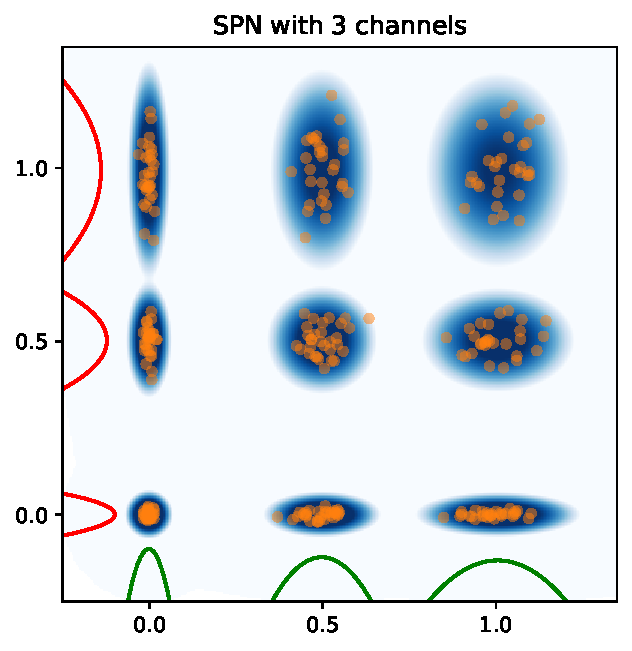
\includegraphics[width=0.46\textwidth]{Pictures/SPN_illustration1.pdf} }%
    \qquad
   {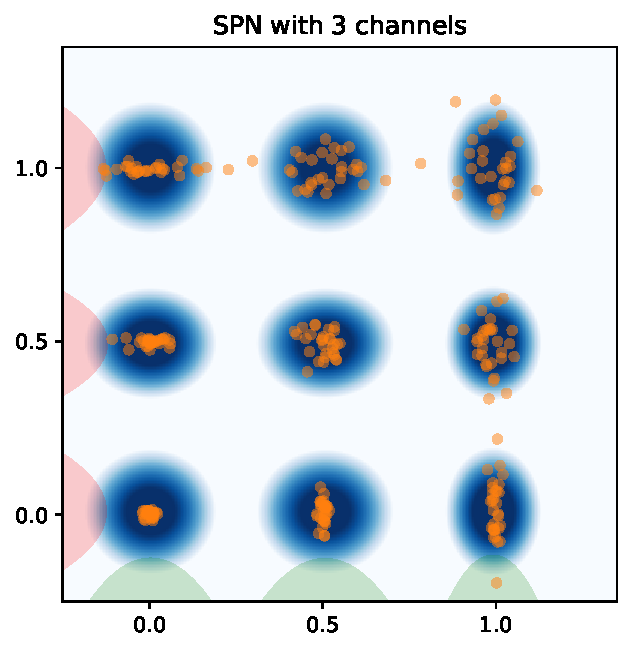
\includegraphics[width=0.46\textwidth]{Pictures/SPN_illustration2.pdf} }%
    \caption{SPN}%
    \label{SPN_fig}%
\end{figure}

\begin{figure}[htbp]
    \centering
    \begin{tikzpicture}

  % Define nodes

   % Define nodes
   \node[latent] (x4) {${x}_4$};
   \node[latent, left=of x4] (x3) {${x}_3$};
   \node[latent, left=of x3] (x2) {${x}_2$};
    \node[latent, left=of x2] (x1) {${x}_1$};
    \node[latent, left=of x1] (x0) {${x}_{0}$};
    
    \node[latent, below=of x4] (x4_hat){$\hat{{x}}_4$};
    \node[obs, below=of x3] (x3_hat){$\hat{{x}}_3$};
    \node[latent, below=of x2] (x2_hat){$\hat{{x}}_2$};
    \node[latent, below=of x1] (x1_hat){$\hat{{x}}_1$};
    \node[obs, below=of x0] (x0_hat){$\hat{{x}}_0$};
    
    \node[const, below= of x2_hat] (sigma-eps) {$\sigma_\epsilon$};
    \node[const, above= of x2] (sigma) {$\sigma$};

%   % Connect the nodes
%    \edge {I-0} {wifi-strength};
    \edge {x1} {x1_hat} ; %
    \edge {x0} {x0_hat} ;
    \edge {x2} {x2_hat} ; %
    \edge {x3} {x3_hat} ;
    \edge {x4} {x4_hat} ; %
    % \edge {a} {sensor-data} ; %

  \edge {x0} {x1} ; %
  \edge {x1} {x2} ; %
  \edge {x2} {x3} ; %
  \edge {x3} {x4} ; %
  
  \edge {sigma} {x1} ; %
  \edge {sigma} {x0}
    \edge {sigma} {x2} ; %
  \edge {sigma} {x3}
    \edge {sigma} {x4} ; %

  \edge {sigma-eps} {x1_hat} ; %
  \edge {sigma-eps} {x0_hat}
   \edge {sigma-eps} {x2_hat} ; %
  \edge {sigma-eps} {x3_hat}
   \edge {sigma-eps} {x4_hat} ; %
%    \plate{} {(wifi-location)(wifi-strength)(wifi-sensor)} {$K$}
%    \plate{} {(x)(x_)(wifi-sensor)(x_hat)} {$T$}
%    \plate{} {(x1)(x0)(x1_hat)} {$T$}    

%   % Plates
%   \plate {yx} {(x)(y)} {$N$} ;
%   \plate {} {(w)(y)(yx.north west)(yx.south west)} {$M$} ;
\end{tikzpicture}
    \caption{Model including wifi information}
    \label{fig:wifi2}
\end{figure}

\begin{figure}[H]
    \centering
    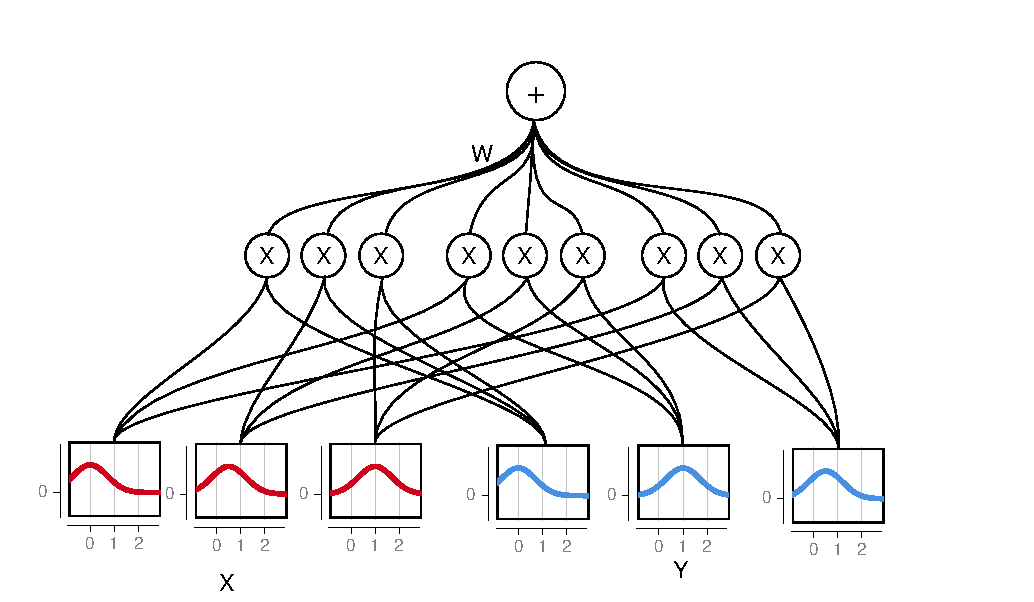
\includegraphics[width=\textwidth]{Figures/SPN_graph2.pdf}
\end{figure}


\section{SPN}
Sum-product networks are generative models, i.e. statistical models of the joint distribution $p(x,y)$. 
We need, however, a disciminative model for regression, i.e. 
a model of the conditional distribution $p(y|x)$. 
SPNs allow for exact inference of the joint distribution 
and any marginalized distribution. These combined queries is sufficient for the
exact predictive posterior. 

\subsection{SPN - prediction}
Prior to the inference of the predictive distribution, we assume that the SPN, S, is trained, i.e.
trained leaf distributions $p_j(\cdot)$ for all leaf nodes, 
$j \in \mathcal{L}eaf(S):=\{j \in \mathcal{V}(S) |pa(j) = \text{Ø}\}$ and
weights $w_{i,j}$ for the connections between every sum nodes
$i \in \mathcal{S}$ and its children, $j \in ch(i)$.  
%The indexes of the nodes, are ordered such that leafs are first, and parents of leafs are next and then the grandparents and so on.

The joint and the marginal distribution are evaluated in the following recursive way
\begin{algorithm}
    \caption*{Calculation of $p(x,y)$}\label{SPN_1}
    \begin{algorithmic}
    \State \textbf{Input:} Fully trained SPN, with leaf distributions $p_i(\cdot)$ for $i\in \mathcal{L}eaf(S)$ and weigts 
    $w_{i,j}$ for $(i,j) \in \{(i,j)|i \in \mathcal{S}um(S), j \in ch(i)\}$ 
    \Function{\text{Eval}}{node i}
    \If{$i \in \mathcal{L}eaf(S)$}
        \State  $\textbf{return: } p_i(x,y)$ \Comment{evaluate leaf distributions at point $(x,y)$}
    \EndIf
    %\For{$i \in I_{o}$}
    \If{$i\in \mathcal{S}um(S)$}
        \State $\textbf{return: } \sum_{j\in ch(i)} w_{i,j} \text{Eval}(j)$
    \EndIf
    \If{$i\in \mathcal{P}rod(S)$}
        \State $\textbf{return: } \prod_{j \in ch(i)} \text{Eval}(j)$
    \EndIf
    \EndFunction
    \State $p(x) =  \text{Eval(root)}$
    \end{algorithmic}
\end{algorithm}

\begin{algorithm}[H]
    \caption*{Calculation of $p(x)$}\label{SPN}
    \begin{algorithmic}
    \State \textbf{Input:} Fully trained SPN, with leaf distributions $p_i(\cdot)$ for all leaves $i$ and weigts $w_{\cdot,\cdot}$ 
    \Function{\text{Eval}}{node i}
    \If{$i \in \mathcal{L}eaf(S)$} %\Comment{leaf node}
        \If{node handle x}
            \State  $\textbf{return: } p_i(x,y)$ \Comment{evaluate leaf distributions at point $(x,y)$}
        \Else 
            \State  $\textbf{return: } 1$ \Comment{set node equal 1 at point $(x,y)$}
        \EndIf
    \EndIf
    \If{$i\in \mathcal{S}um(S)$}
        \State $\textbf{return: } \sum_{j\in ch(i)} w_{i,j} \text{Eval}(j)$
    \EndIf
    \If{$i\in \mathcal{P}rod(S)$}
        \State $\textbf{return: } \prod_{j \in ch(i)} \text{Eval}(j)$
    \EndIf
    \EndFunction
    \State $p(x) =  \text{Eval(root)}$
    \end{algorithmic}
\end{algorithm}

So after doing two slightly different forward passes through the SPN, 
$p(x)$ and $p(x,y)$, using Bayes rule,
we can combined the two queries into the conditional distribution: 
$$p(y|x) = \frac{p(x,y)}{p(x)}$$
The predictive distribution is found with a cost of just $O(E+E+1) = O(E)$, where E is number
of edges/connections in the SPN. 

\subsection{SPN - learning}
It is not enouth to do predictive inference on a SPN, we also need to fit it on
the data. It is possible interpret sum-product network as a large mixture model 
and therefore use expectation-maximization to train the model. 
We will introduce that idea now. The Paper \cite{SPN_EM}... %["Learning Arbitrary Sum-Product Network Leaves
%with Expectation-Maximization"] 
defines SPN as a mixture of all sub-networks of an SPN.

%from [@desana]:
\begin{definition} 
    A sub-network $\bar S_z$ of $S$ is an SPN, which includes the root $S$ and then includes nodes
    according to the following recursive scheme: 
\end{definition}
\begin{algorithm}[H]
    \caption*{Collection of sub-network $S_z$ of $S$}\label{SPN3}
    \begin{algorithmic}
    %\State \textbf{Global:}  $S_z$ 
    \Function{Process}{node i, $S_z$}
    \If{$i \in \mathcal{L}eaf(S)$}
        \State  $\textbf{return: }$ 
    \EndIf
    %\For{$i \in I_{o}$}
    \If{$i\in \mathcal{S}um(S)$}
       %\State $S_z =S_z \cup \{j \in ch(i)\}$ \Comment{include one child of node $i$}
        \State $S_z =S_z.add(j \in ch(i))$ \Comment{include one child of node $i$}
        \State $\textbf{return: } \text{Process}(j, S_z)$
    \EndIf
    \If{$i\in \mathcal{P}rod(S)$}
        \State $S_z =S_z \cup \{j | j \in ch(i)\}$ \Comment{include all childen of node $i$}
        \For{$j \in ch(i)$}
            \State $\textbf{return: } \text{Process}(j,S_z)$
        \EndFor
    \EndIf
    \State $\textbf{return: } S_z$
    \EndFunction
    \State $S_z =  \text{Process(root,Ø)}$
    \end{algorithmic}
\end{algorithm}
So we see that at each sum node the number of different sub-networks multiplies with the number of children for that
sum node. And thereby, the total number of sub-networks is
 $$Z = \prod_{i\in \mathcal{S}um(S)}|ch(i)|$$ 
 i.e. an exponential large amount of sub-networks. This is the amount of
 mixture components implicitly defined in an SPN. 
 Denote the set of edges in the sub-network $\mathcal{E}(S_z)$.
Now the we define a mixture coeficient, $\lambda_z$ and component for each $S_z$ as 
$$\lambda_z := \prod_{(i,j)\in \mathcal{E}(S_z)} w_{i,j}, \hspace{1cm}
p_z(x,y|\theta) := \prod_{i \in \mathcal{L}(S_z)} p_i(x,y)$$
where $p_i(x,y)$ is the leaf distribution at leaf node $i$ paramitised with $\theta$. 
It can now be proven that the SPN can be interpreted as the following mixture model, 
$$p(x,y|w,\theta) = \sum_{z=1}^Z \lambda_z(w)p_z(x,y|\theta)$$
i.e. by the weighted sum of all $Z$ sub-networks. For convinience
we define each sum component as $p(z,x,y|w,\theta) := \lambda_z(w)p_z(x,y|\theta)$.
Evaluation of $p(x,y|w,\theta)$ will never be done as the sum over $Z$ components, 
instead there is a proposition. 

\begin{proposition}
    Consider a SPN, S, a sum node $q \in \mathcal{S}um(S)$ and a child $i \in ch(q)$,
    then the following relation holds, 
    $$\sum_{z:(q,i)\in \mathcal{E}(S_z)} \lambda_z(w) p_z(x,y|\theta) = w_{i,q}
    \frac{\partial S}{\partial v(q)} v(i)$$
\end{proposition}

\newpage
\section{Expectation-maximization for mixture models}
Mixture models can be seen as probibalistic graphical models, <fig> there one mixture component is
picked according to the realization of a catagorical variable $\textbf{Z}$ with parameters according
the the mixture weights, i.e we can reformelate, 
\begin{align}\label{mixture_pdf}
    p(x) &= \sum_{k=1}^K w_k p_k(x)\\
   \iff \hspace*{1cm} p(x) &= p_z(x), \hspace*{0.5cm} z \sim Cat(w_i, \dots, w_K).
\end{align}
In fact $p_z(x)$ is a conditial distribution, $p(x|z)$, and combined with the distribution
of $Z$ we can define the joint 
$$p(x,z):=p_z(x)p(z)$$
The the case of a statistical model, data $\mathcal{D}$ is fitted by the mixture model 
by tuning the model parameters $\theta = \{w, \text{paramers for} p_i\}$. Then the joint
distribtuion $p(\mathcal{D},z| \theta)$ is refered as the \textit{complete-data} likehood in the EM algorithm. 
$$p(\mathcal{D},z|\theta):=p(\mathcal{D}|z,\theta)p(z|\theta)$$ 
When fitting model parameters we essentially want to find the parameters, that maximize the probability of
the parameters given the data, $p(\theta|\mathcal{D})$. Assuming an
unimformative/flat prior $p(\theta)$, 
\begin{align*}
p(\theta|\mathcal{D})&= \frac{p(\mathcal{D}|\theta)p(\theta)}{p(\mathcal{D})}\\
\Rightarrow  \arg\max_{\theta} p(\theta|\mathcal{D}) &= \arg\max_{\theta} p(\mathcal{D}|\theta)
\end{align*}
we arrive at the maximum likelihood estimate (MLE). The task of finding the MLE is conviniently
done using EM algorithm, since we can look at the likehood as the marginalized
\textit{complete-data} likehood, 
$$p(\mathcal{D}|\theta) = \sum_z p(\mathcal{D}, z|\theta)$$

%(Note that this statement true accoring to Theorem 2.1. in \cite{gupta2011theory}). 

\begin{testexample2}[Expectation-maximization EM <based on \cite{bishop}]
    Expectation maximization is a convinient method for finding ML (or MAP) estimate of a 
    latent variable model. We consider a probibalistic model paramitised with $\theta$, 
    $$p(\textbf{X}, \textbf{Z}|\theta)$$ where we denote all latent variables \textbf{Z}, and
    observed variables \textbf{X}. Our goal is to find the maximum of the likehood, 
    $$p(\textbf{X}|\theta) = \int p(\textbf{X}, \textbf{Z}| \theta) \mu(d\textbf{Z})$$
    maximizating the likehood itself $p(\textbf{X}|\theta)$ is assumed dificult 
    but maximizating of the \textit{complete-data} likehood $p(\textbf{X}, \textbf{Z}|\theta)$
    is much easier. The algorithm iterates over two steps: The expecation (E) step and the maximization (M) step, 
    defined in the following way for iteration $t$, 
    
    \textbf{E-step}

    Define the functional $Q(\theta,\theta^{(t)})$, to be the expected value of the complete-data 
    log likehood (log likehood function of $\theta$), with respect to the only random quantaty $\textbf{Z}$,
    which is assumed to follow a distribtuion with the density $p(\textbf{Z}|\textbf{X}, \theta^{(t)})$,
    i.e. the conditional distribution of \textbf{Z} given \textbf{X} and the current parameter point estimate
    $\theta^{(t)}$: 
    $$Q(\theta,\theta^{(t)}) := E_{p(\textbf{Z}|\textbf{X}, \theta^{(t)})}[\log p(\textbf{X}, \textbf{Z}|\theta)]$$

    \textbf{M-step}

    After the E-step we find the point estimate $\theta^{(t+1)}$ which maximizes $Q(\cdot|\theta^{(t)})$, i.e.
    $$\theta^{(t+1)} = \arg\max_{\theta} Q(\theta|\theta^{(t)})$$

    \begin{algorithm}[H]
        \caption*{(local) maximization of $p(\mathcal{D}|\theta)$}\label{EM}
        \begin{algorithmic}
        \State \textbf{Input:} dataset $\mathcal{D}$, joint model $p(\mathcal{D}, \textbf{Z}|\theta)$
        \While{Not converged}
            \State $Q(\cdot, \theta^{(t)}) \gets E_{p(\textbf{Z}|\mathcal{D}, \theta^{(t)})}[\log p(\mathcal{D}, \textbf{Z}|\cdot)]$ \Comment{E-step}
            \State $\theta^{(t+1)} \gets \arg\max_{\theta} Q(\theta|\theta^{(t)})$ \Comment{M-step}
        \EndWhile
        \State $\textbf{return: } \theta^{(end)}$
    \end{algorithmic}
    \end{algorithm}

    \textbf{Proof of correctness} 
    
    We will now give a short proof that maximizing $Q(\cdot|\theta^{(t)})$ maximizes the likelihood
    $p(\textbf{X}|\theta)$, where we assume that $\textbf{Z}$ is a random vector with a discrete
    distribution. This allow us to use Gibbs inequality: 
    $$\sum_z p_1(z) \log p_1(z) \geq \sum_z p_1(z) \log p_2(z)$$ where $p_1(\cdot)$ and $p_2(\cdot)$
    are densities belonging to two discrete distributions of $Z$, equality if $p_1(\cdot) =
    p_2(\cdot)$. From now on we will alter the subscript on the expecations, just have in mind that
    $$E_{\theta^{(t)}}[g(Z)]:=E_{p(\textbf{Z}|\textbf{X}, \theta^{(t)})}[g(Z)] = \sum_z g(z)
    p(\textbf{z}|\textbf{X}, \theta^{(t)})$$ 
    Now to the proof: From bayes rule $p(\textbf{X}|\theta) =
    \frac{p(\textbf{X}, \textbf{Z})}{p(\textbf{X})}$ we can write
    $$\log p(\textbf{X}|\theta) = \log p(\textbf{X}, \textbf{Z}) - \log p(\textbf{Z}|\textbf{X},\theta)$$
    Now, taking the expecation of the above w.r.t. $p(\textbf{Z}|\textbf{X}, \theta^{(t)})$,
    yields,
    \begin{align*}
        \log p(\textbf{X}|\theta)  &= E_{\theta^{(t)}}[\log p(\textbf{X}, \textbf{Z}|\theta)]
        -  E_{\theta^{(t)}}[\log p(\textbf{Z}|\textbf{X},\theta)]\\
        &= Q(\theta,\theta^{(t)})+ E_{\theta^{(t)}}[\log p(\textbf{Z}|\textbf{X},\theta)]
    \end{align*} 
    Since the above equation holds for any $\theta$, it also holds for $\theta^{(t)}$
    now we have, 
    $$\log p(\textbf{X}|\theta^{(t)}) = Q(\theta^{(t)},\theta^{(t)})+ E_{\theta^{(t)}}[\log
    p(\textbf{Z}|\textbf{X},\theta^{(t)})]$$ 
    Subtracting the two equations, we get,  
    $$\log p(\textbf{X}|\theta) - \log p(\textbf{X}|\theta^{(t)}) = Q(\theta,\theta^{(t)})
    -Q(\theta^{(t)},\theta^{(t)})+ E_{\theta^{(t)}}[\log p(\textbf{Z}|\textbf{X},\theta)]-
    E_{\theta^{(t)}}[\log p(\textbf{Z}|\textbf{X},\theta^{(t)})]$$ 
    From Gibb's inequality we have
    that $E_{\theta^{(t)}}[\log p(\textbf{Z}|\textbf{X},\theta^{(t)})]\leq E_{\theta^{(t)}}[\log
    p(\textbf{Z}|\textbf{X},\theta)]$ where equality only holds for $\theta^{(t)} = \theta$, giving
    \begin{align*}
        \log p(\textbf{X}|\theta) - \log p(\textbf{X}|\theta^{(t)}) \geq 
    Q(\theta,\theta^{(t)})
    -Q(\theta^{(t)},\theta^{(t)})
    \end{align*}
    so optimizing $Q(\theta,\theta^{(t)})$ will optimize
    $\log p(\textbf{X}|\theta) $ as least as much.
\end{testexample2}

 \subsection*{EM for Gaussian mixture}
 For a Gaussian mixture the $p_k$ distributions in \eqref{mixture_pdf} is substituted by Gaussain pdfs, 
 i.e. $p_k(x) = \mathcal{N}(x| \mu_k , \Sigma_k)$
 and the density of a catagorical distribution is $p(z) = \sum_{k=1}^K 1_{z=k} w_k = w_z$, combining the two
 we get the joint distribution, 
 $$p(x,z|w,\mu , \Sigma) = w_z \mathcal{N}(x| \mu_z , \Sigma_z)$$

 Taking the log and defning $\theta = \{\mu_1 , \Sigma_1,w_1, \dots, \mu_K , \Sigma_K, w_K\}$, and assuming iid data
 $$\log p(X,Z| \theta) = \sum_{i}^n \left(\log(w_{z_i})+\log(\mathcal{N}(x_i| \mu_{z_i} , \sigma_{z_i}))\right)$$

Now we are ready to calculate $Q(\theta, \theta^{(t)})$, by taking the expectation of the complete-data log likehood
with respect to the distribution, $p(Z|X, \theta)$, 
\begin{align*}
    E_{p(Z|X,  \theta^{(t)})}[\log p(X,Z| \theta)] &=\sum_{i}^n  E_{p(Z|X,  \theta^{(t)})}[p(X_i,Z_i| \theta) ]\\
    &=\sum_{i}^n  E_{p(z_i|x_i,  \theta^{(t)})}[p(x_i,z_i| \theta) ]
\end{align*}

\begin{tcolorbox}[
    sharp corners,
    boxrule=0mm,
    enhanced,
    borderline west={4pt}{0pt}{gray},
    colframe=drGray,
    colback=drGray,
    coltitle=black,
]
{\large \textbf{Expectation with repect to unnecessary variables}}\\
the last equation holds since taking expecation over a function of a random variable $x$ with respect to a that random
variable and more random variabels, $x,y$, is equivalent to the expecation with respect to just $x$, i.e. 
\begin{align*}
    E_{x,y}[g(x)] &= \int\int g(x) p(x,y) dy dx\\
     &= \int g(x) \int p(x,y) dy dx \\
    &= \int g(x) p(x) dy = E_x[g(x)]
\end{align*}
\end{tcolorbox}

the posterior distribution is calculated the following way,
\begin{align*}
    p(z|x, \theta^{(t)}) &= \frac{p(x,z|\theta^{(t)})}{p(x|\theta^{(t)})} \\
    &= \frac{p(x,z|\theta^{(t)})}{\sum_{z} p(x,z|\theta^{(t)})}\\
    &= \frac{w_z^{(t)} \mathcal{N}(x|\mu_z^{(t)}, \Sigma_z^{(t)})}{\sum_{k=1}^K w_k^{(t)} 
    \mathcal{N}(x|\mu_k^{(t)}, \Sigma_k^{(t)})}
\end{align*}
For simplificaiton we will denote, $\gamma^{(t)}(z_i) := p(z_i|x_i, \theta^{(t)})$, 
interpreted as the probability of datapoint $x_i$ to belong to class $z_i$. Bishop \cite*{bishop}
calls this probability function the \textit{responsibility}. We can now conclude the \textbf{E-step}.

\begin{align*}
    Q(\cdot, \theta^{(t)}) &= \sum_{i=1}^n p(x_i,z_i|\cdot) \gamma^{(t)}(z_i) \\
    &= \sum_{i=1}^n \left[ \gamma^{(t)}(z_i) \log(\cdot_{z_i})+\gamma^{(t)}(z_i) 
    \log(\mathcal{N}(x_i| \cdot_{z_i} , \cdot_{z_i}))\right]
\end{align*}
or more concretely $\theta = \{\mu_1 , \Sigma_1,w_1, \dots, \mu_K , \Sigma_K, w_K\}$, 
$$ Q(\theta, \theta^{(t)}) = \sum_{i=1}^n \gamma^{(t)}(z_i) \log(w_{z_i})+\gamma^{(t)}(z_i) \log(\mathcal{N}(x_i| \mu_{z_i} , \Sigma_{z_i})).$$
$Q(\cdot, \theta^{(t)})$ is a concave function - the Gaussian is log-concave and a sum of concave functions is 
also concave - so it is sufficient and nessesary to find its maxima by the root of its derivative, 
$$\frac{d}{d \theta} Q(\theta^*, \theta^{(t)}) = 0 \iff \theta^* = \arg\max_{\theta} Q(\theta, \theta^{(t)})$$

Giving the updates...

\subsection*{EM for SPN}


% and a normal evaluation of $p(x,y|w_{old}, \theta_{old})$ combined in Bayes rule we obtain
% $$p(z|x,y,w_{old},\theta_{old}) = \frac{p(z,x,y|w_{old},\theta_{old})}{p(x,y|w_{old},
% \theta_{old})} = \frac{\lambda_z(w_{old})p_z(x,y|\theta_{old})}{p(x,y|w_{old}, \theta_{old})} $$

% and we have the expecation for the EM-algorithm, 
% $$Q(\pi, \pi_{old}) = \sum_{n=1}^N \sum_{z=1}^Z p(z|xy_n, \pi_{old}) \ln p(z,xy_n|\pi)$$


\section{Gaussian Mixture Regression}
The Gaussian mixture is a generative model of the joint probability of $x$ and $y$ given as, 
$$p(x,y)= \sum_{k=1}^K \pi^{(k)} \mathcal{N}(x,y|\mu^{(k)},\Sigma^{(k)}), 
\hspace{1cm} \mu=\begin{bmatrix}
    \mu_x \\ \mu_y
\end{bmatrix},\hspace{0.1cm} \Sigma = \begin{bmatrix}
    \Sigma_{xx} & \Sigma_{xy}\\ \Sigma_{yx}& \Sigma_{yy}
\end{bmatrix}$$
This is trained using the EM algorithm. We will now show how the conditial is
calculated exact. 
\subsection{GMR - prediction}
We need the conditional distribution of the Gaussian mixture
in order to get the predictive distribution. We will now formulate
the conditial distribution in terms of conditional and marginals of
the individual mixture components. First of all the marginal distribution $p(x)$ 
of the mixture is given as, \todo{How??!}
$$p(x) = \sum_{k=1}^K \mathcal{N}(x|\mu_{x}^{(k)},\Sigma_{xx}^{(k)})$$ 
next the joint distribution can be decomposed with the probability chain rule,
\begin{align*}
    p(x,y) &= p(x)p(y|x)\\
    \implies \hspace{1cm} \mathcal{N}(x,y|\mu,\Sigma) &= 
    \mathcal{N}(x|\mu_{x},\Sigma_{xx}) \mathcal{N}(y|\mu_{y|x},\Sigma_{y|x})
\end{align*} 
And we can formulate the conditial in terms of individual multivariate Gaussians, 

\begin{align}
    p(y|x) &= \frac{p(y,x)}{p(x)}\\
    &= \sum_{k=1}^K \frac{\pi^{(k)}}{p(x)} \mathcal{N}(x,y|\mu^{(k)},\Sigma^{(k)})\\
    &=  \sum_{k=1}^K \frac{\pi^{(k)} \mathcal{N}(x|\mu_{x}^{(k)},\Sigma_{xx}^{(k)})}{p(x)}\mathcal{N}(y|\mu_{y|x}^{(k)},\Sigma_{y|x}^{(k)})\\
    &=  \sum_{k=1}^K \pi_{y|x}^{(k)} p(y|x,\mu_{y|x}^{(k)},\Sigma_{y|x}^{(k)})
\end{align}

where $\pi_{y|x}^{(k)} := \frac{\pi^{(k)} \mathcal{N}(x|\mu_{x}^{(k)},\Sigma_{xx}^{(k)})}
{\sum_{i=1}^K \mathcal{N}(x|\mu_{x}^{(i)},\Sigma_{xx}^{(i)})}$. So we see that 
the conditonal of a Gaussian mixture model is again a Gaussian mixture model.


\begin{testexample2}[Conditional og multivariate Gaussian]
    The conditional distribution is defined as \cite{bishop} ..?
    $$p(y|x,\mu, \Sigma) = \mathcal{N}(y|\mu_{y|x},\Sigma_{y|x} )\hspace{1cm} \mu=\begin{bmatrix}
        \mu_x \\ \mu_y
    \end{bmatrix},\hspace{0.1cm} \Sigma = \begin{bmatrix}
        \Sigma_{xx} & \Sigma_{xy}\\ \Sigma_{yx}& \Sigma_{yy}
    \end{bmatrix}$$ 
    where 
    \begin{align}
        \mu_{y|x} &= \mu_y+\Sigma_{yx}\Sigma_{xx}^{-1}(x-\mu_x)\\
        \Sigma_{y|x} &= \Sigma_{yy}-\Sigma_{yx}\Sigma_{xx}^{-1}\Sigma_{xy} 
    \end{align}
    
\end{testexample2}


\subsection{GMR - Leaning}

EM-algorithm, classic example. 